%! Author = chtompki
%! Date = 1/14/26
% Example LaTeX document for GP111 - note % sign indicates a comment
\documentclass[12pt]{amsart}
% Default margins are too wide all the way around. I reset them here
\setlength{\hoffset}{-.75in}
\setlength{\textwidth}{6.5in}
\setlength{\voffset}{-.5in}
\setlength{\textheight}{9.0in}
\usepackage{amsmath}
\usepackage{amssymb}
\usepackage{amsthm}
\usepackage{pgfplots}
\usepackage{enumerate}
\usepackage{tikz}
\usetikzlibrary{shadows,arrows,arrows.meta,shapes,positioning,calc}% Required for the Circle and Triangle arrow tips
\usepackage{setspace}
\usepackage{siunitx}

\theoremstyle{definition}
\newtheorem{definition}{Definition}

\title{Seminar Summary:\\February 17, 2026 - Marco Aldi\\NP Problems and their Quantum Analogues}
\author{Rob Tompkins}
\date{\today}


\begin{document}
    \maketitle
    \date{\today}
    \begin{onehalfspace}
        Anything that can be calculated on today's computers could have been calculated using mechanical machine.
        An example of a particularly sophisticated calculating machine was established by Babbage.
        In fact anything calculable with one of the most sophisticated computers today (quantum aside) could be
        worked out by hand in a step-by-step process with boundaries given for input and a sufficient set of
        instructions.
        These mechanical calculators or computers as we call them, are particularly good at solving a particular
        set of problems.
        These are the easy problems with which we are familiar, alphabetizing a list,
        finding the value of an element in a list, merging two lists, and many more.
        Though things become difficult when we are asked if an arbitrary collection of integers contains a subset that
        sums to zero.
        Moreover, it is even harder to find that subset.
        Note, there are a collection of problems that are essentially analogous this problem about finding a subset of
        integers that sums to zero.

        In the early 1970's, 1971 to be exact, Stephen Cook and Leonid Levin independently went about attempting to
        formally define the characteristic to a problem that lands it in one of these two categories.
        The easier first collection of problems are those that given an input of length $n$ can be solved in
        $n^k + a$ steps with $a,k\in\mathbb{N}$.
        These problems we call \emph{polynomial time} problems because they can be solved in $\mathcal{O}(n^k)$ steps
        the problem space $\mathbf{P}$.

        Then there are problems that are known to take a substantial amount of time, for example exhaustive
        search for a directory in a large un-indexed directory tree.
        These problems are known to take $\mathcal{O}(2^n)$ steps, or \emph{exponential time}.

        Now, these inbetween difficulties problems.
        How are we to classify them.
        Originally, we were concerned with polynomial time algorithms over a Non-deterministic Turing Machine.
        Where a Non-deterministic Turing Machine is one that given a tape position and a state, one has multiple next states
        into which to move, which leaves us with a relatively vague yet faster path to our solution.
        Eventually people became impatient with the vagueness of this definition, and the following definition arose.

        \begin{definition}
            (The class $\mathbf{NP}$) A language $L\subseteq\{0,1\}^*$ (the kleene closure over $\{0,1\}$) is in
            $\mathbf{NP}$ provided there exists a polynomial $p:\mathbb{N}\rightarrow\mathbb{N}$ and a polynomial-time
            turing machine $M$ (called the \emph{verifier} of $L$) such that for every $x\in\{0,1\}^*$
            \begin{displaymath}
                x\in L \Leftrightarrow \exists u\in\{0,1\}^{p(|x|)}\quad\text{s.t.}\quad M(x,u)=1.
            \end{displaymath}
            If $x\in L$ and $u\in\{0,1\}^{p(|x|)}$ satisfy $M(x,u)=1$, then we call $u$ a \emph{certificate} for $x$
            (with respect to the language $L$ and the machine $M$).
        \end{definition}

        \noindent\textbf{Question.} Does $\mathbf{P} = \mathbf{NP}$?\\

        Over the years multiple different fields have all made their own progress on the problem.
        Figure \ref{figureFields} gives us a venn-diagram of some of the more important fields involved in
        making progress on $\mathbf{NP}$-hard problems, whether $\mathbf{P}$ and $\mathbf{NP}$ are the same set of problems.

        \begin{figure}
            \centering
            \begin{tikzpicture}[scale=1, line width=0.9pt]

    % --- centers (tuned so CC overlaps AA) ---
                \coordinate (Cc) at (-1.8,0.6);   % Computational Complexity (moved right)
                \coordinate (Cr) at ( 2.0,0.2);   % Abstract Algebra (moved left)
                \coordinate (Cd) at ( 0.2,-2.1);  % Discrete Math
                \coordinate (Cp) at ( 0.7,0.9);   % Physics (ellipse center)

    % --- radii ---
                \def\Rc{2.45}
                \def\Rr{2.15}
                \def\Rd{2.55}

    % Physics ellipse shape
                \def\a{0.95}   % x-radius
                \def\b{2.75}   % y-radius
                \def\ang{-18}   % rotation

    % --- shaded region: Physics ∩ Discrete ∩ Abstract (edit if you want all 4) ---
                % --- shaded region: intersection of ALL FOUR ---
                \begin{scope}
                    \clip (Cc) circle ({\Rc});  % Computational Complexity
                    \clip (Cr) circle ({\Rr});  % Abstract Algebra
                    \clip (Cd) circle ({\Rd});  % Discrete Math
                    \clip[rotate around={\ang:(Cp)}] (Cp) ellipse ({\a} and {\b}); % Physics
                    \fill[black!70] (-10,-10) rectangle (10,10);
                \end{scope}

    % --- outlines ---
                \draw (Cc) circle ({\Rc});
                \draw (Cd) circle ({\Rd});
                \draw (Cr) circle ({\Rr});
                \draw[rotate around={\ang:(Cp)}] (Cp) ellipse ({\a} and {\b});

    % --- labels ---
                \node[align=center] at ($(Cc)+(0,0.3)$) {Computational\\Complexity};
                \node[align=center] at ($(Cd)+(0,-0.15)$) {Discrete\\Math};
                \node[align=center] at ($(Cr)+(0.2,0.35)$) {Abstract\\Algebra};
                \node at (1.35,3.88) {Physics};

            \end{tikzpicture}
            \caption{Fields involved in making progress on $\mathbf{NP}$-hard problem research}
            \label{figureFields}
        \end{figure}

        Now that we have the class of $\mathbf{NP}$-hard problems, it becomes important to have an example
        of an $\mathbf{NP}$-hard problem.
        Now we earlier mentioned the integer subset sum problem, but this was not the original problem proven to
        be $NP$-hard.
        That was the boolean satisfaction problem, ``SAT''.
        SAT is defined by considering a list of variables $s_0,s_1,\ldots,s_{n-1} \in\{0,1\}$ and a function
        $f:\{0,1\}^n\rightarrow\{0,1\}$, find the answer to $f(s_0,s_1,\ldots,s_{n-1}) = 0$ (or 1).
        We can think of $f$ as an arbitrary list of and's $\land$ and or's $\lor$, with our $s$'s as variables,
        and we are trying to find a solution that yields \emph{true}.
        Clearly finding a solution is quite difficult, but checking if a collection of $s$'s is a solution is an answer
        is as easy as plugging them into $f$, a polynomial-time task.
        Oddly, every \emph{known} $\mathbf{NP}$-hard problem reduces to SAT, and we call these problems
        $\mathbf{NP}$-complete.
        Four classical examples of problems that are $NP$-complete are: the Hamiltonian Path problem, 3SAT (the boolean
        satisfaction problem factored into 3 blocs of ands or'd together or vice versa), the Independent Set Problem,
        and the Travelling Salesman Problem.

        We went over the definition of the Independent Set problem (which personally I had not seen before and found
        quite interesting).
        We consider graphs of the form given in Figure \ref{figureIndepSet}, and the following definition.
        \begin{definition}
            A subset of vertices $S\subseteq V$ in a graph $G = (V,E)$ is an \emph{independent set} for all $u,v\in S$
            if the edge $\{u,v\}\notin E$.
        \end{definition}
        The decision problem is stated as: given a graph $G$ and $k\in\mathbb{Z}$, does $G$ contain an independent set
        of size$\;\ge k$?

        \begin{figure}
            \centering
            \begin{tikzpicture}[line width=0.9pt, scale=1,
                vertex/.style={circle, fill=black, inner sep=1.6pt}
            ]

% --- coordinates (tweak if you want different proportions) ---
                \coordinate (T)  at (0,3.6);      % top junction of the Y
                \coordinate (L1) at (-1.6,5.2);   % top-left end
                \coordinate (R1) at ( 1.6,5.2);   % top-right end

                \coordinate (M)  at (0,1.8);      % middle junction on the vertical
                \coordinate (A)  at (0,0.9);      % triangle apex (same as M? no, small drop)

                \coordinate (BL) at (-1.7,-0.4);  % triangle base left
                \coordinate (BR) at ( 1.7,-0.4);  % triangle base right (also junction to tail)
                \coordinate (D)  at ( 1.7,-2.6);  % bottom of the tail

% --- edges ---
                \draw (L1)--(T)--(R1);   % top Y arms
                \draw (T)--(M);          % vertical down from top junction

                \draw (M)--(BL)--(BR)--cycle; % triangle (M is the apex)
                \draw (BR)--(D);              % tail down from bottom-right vertex

% --- intersection points (vertices) ---
                \node[vertex] at (T)  {};
                \node[vertex] at (M)  {};
                \node[vertex] at (BL) {};
                \node[vertex] at (BR) {};

            \end{tikzpicture}
            \caption{A graph}
            \label{figureIndepSet}
        \end{figure}

        \section{Quantum Computing}
    \end{onehalfspace}
\end{document}
